% Mario Guerra Castelo

\begin{table}[h]
    \centering
    \begin{tabular}{lr}
        \textbf{Cuenta de Resultados - 2ª Decisión} & \textbf{€} \\
        \hline
        \textbf{Ingresos por ventas}                & \textbf{601815} \\
        Valor Stock inicial                         & 315017 \\
        Componentes comprados                       & 24570 \\
        Adquisición de materias primas              & 636306 \\
        Funcionamiento máquinas                     & 54624 \\
        Salarios mecanizado                         & 123302 \\
        Salarios montaje                            & 61009 \\
        Control de calidad                          & 1241 \\
        Transporte                                  & 18400 \\
        Menos valor de stock final                  & 691272 \\
        \cline{2-2}
        \textbf{Coste de las ventas}                & 543197 \\
        \cline{2-2}
        \textbf{Beneficio Bruto}                    & 58618 \\
        Gastos generales                            & 619803 \\
        Seguros recibidos                           & 39781 \\
        Amortización                                & 26102 \\
        \cline{2-2}
        \textbf{EBIT}                               & -547506 \\
        Ingresos financieros                        & 500 \\
        \textbf{Gastos financieros}                 & \textbf{0} \\
        \cline{2-2}
        \textbf{Beneficio antes de impuestos}       & \textbf{-547006} \\
        Impuestos                                   & 0 \\
        \cline{2-2}
        \textbf{Resultado neto}                     & \textbf{-547006} \\
        \textbf{Beneficio por acción (cents)}       & \textbf{-13,67515} \\
        \textbf{Pago de dividendos}                 & \textbf{0} \\
        \cline{2-2}
        Transferido a reservas                      & -547006 \\
        Reservas acumuladas                         & -229654 \\
        \cline{2-2}
        \textbf{Reservas totales}                   & \textbf{-776660}
    \end{tabular}
\end{table}

\begin{table}[h]
    \centering
    \begin{tabular}{|c|r|}
        \hline
        Margen Explotación  & -90,98 \% \\
        Margen Operativo    & -90,89 \% \\
        Margen Neto         & -90,89 \% \\
        ROA                 & -14,13 \% \\
        ROE                 & -16,97 \% \\
        Rotación            & 15,72 \% \\
        Endeudamiento       & 18,80 \% \\
        \hline
    \end{tabular}
\end{table}

\section*{Trimestre 4, el inicio del declive}
El cuarto trimestre de 2017 será recordado como el periodo en el que la desconexión entre el departamento comercial y el de operaciones llevó a IndusMoney a una situación de vulnerabilidad financiera. A pesar de que los indicadores macroeconómicos sugerían una oportunidad de expansión, la empresa experimentó una caída en la facturación del 50,7\% (pasando de 1,22M€ a 601K€). 

Este declive no se debe a una falta de competitividad del producto o a un rechazo del mercado, sino a una parálisis operativa autoinfligida. La empresa generó una demanda que no pudo atender, lo que resultó en un margen bruto de apenas el 9,74\%, insuficiente para cubrir una estructura de gastos fijos y de marketing que se diseñó para un volumen de ventas tres veces mayor. La consecuencia directa ha sido una pérdida neta superior al medio millón de euros, drenando la caja y debilitando el balance justo antes del cierre del año fiscal. 

\section*{Radiografía del descalabro}
El dato más alarmante del T7 es el resultado neto, con una pérdida de -547.006€. Esta cifra no solo erosiona el patrimonio neto de la empresa, sino que sitúa a la compañía en una posición de vulnerabilidad extrema. 

Las ventas se hundieron hasta los 601.815€, una caída del 50,7\% respecto al trimestre anterior. Este descenso no responde a una falta de demanda en el mercado, sino a una incapacidad absoluta de suministro. 

Con unos ingresos tan reducidos, el margen bruto no alcanza siquiera para cubrir los gastos fijos de estructura. La empresa está operando por debajo de su punto de equilibrio. 

El flujo de caja neto fue de -323.116€. A pesar de contar con un saldo de caja de 1,5 millones (gracias a la prudencia de trimestres anteriores), este ritmo de consumo de efectivo es insostenible a medio plazo. 

\section*{La Paradoja del Marketing y la Ruptura de Stock}
La raíz de este retroceso financiero se encuentra en una decisión de producción extremadamente conservadora que chocó frontalmente con una estrategia de ventas expansiva. En el Trimestre 6, la empresa fabricó 1.350 unidades del Producto 1; sin embargo, para este trimestre, la programación se desplomó a solo 471 unidades (un recorte del 65\%).

\begin{figure}[h]
  \centering
  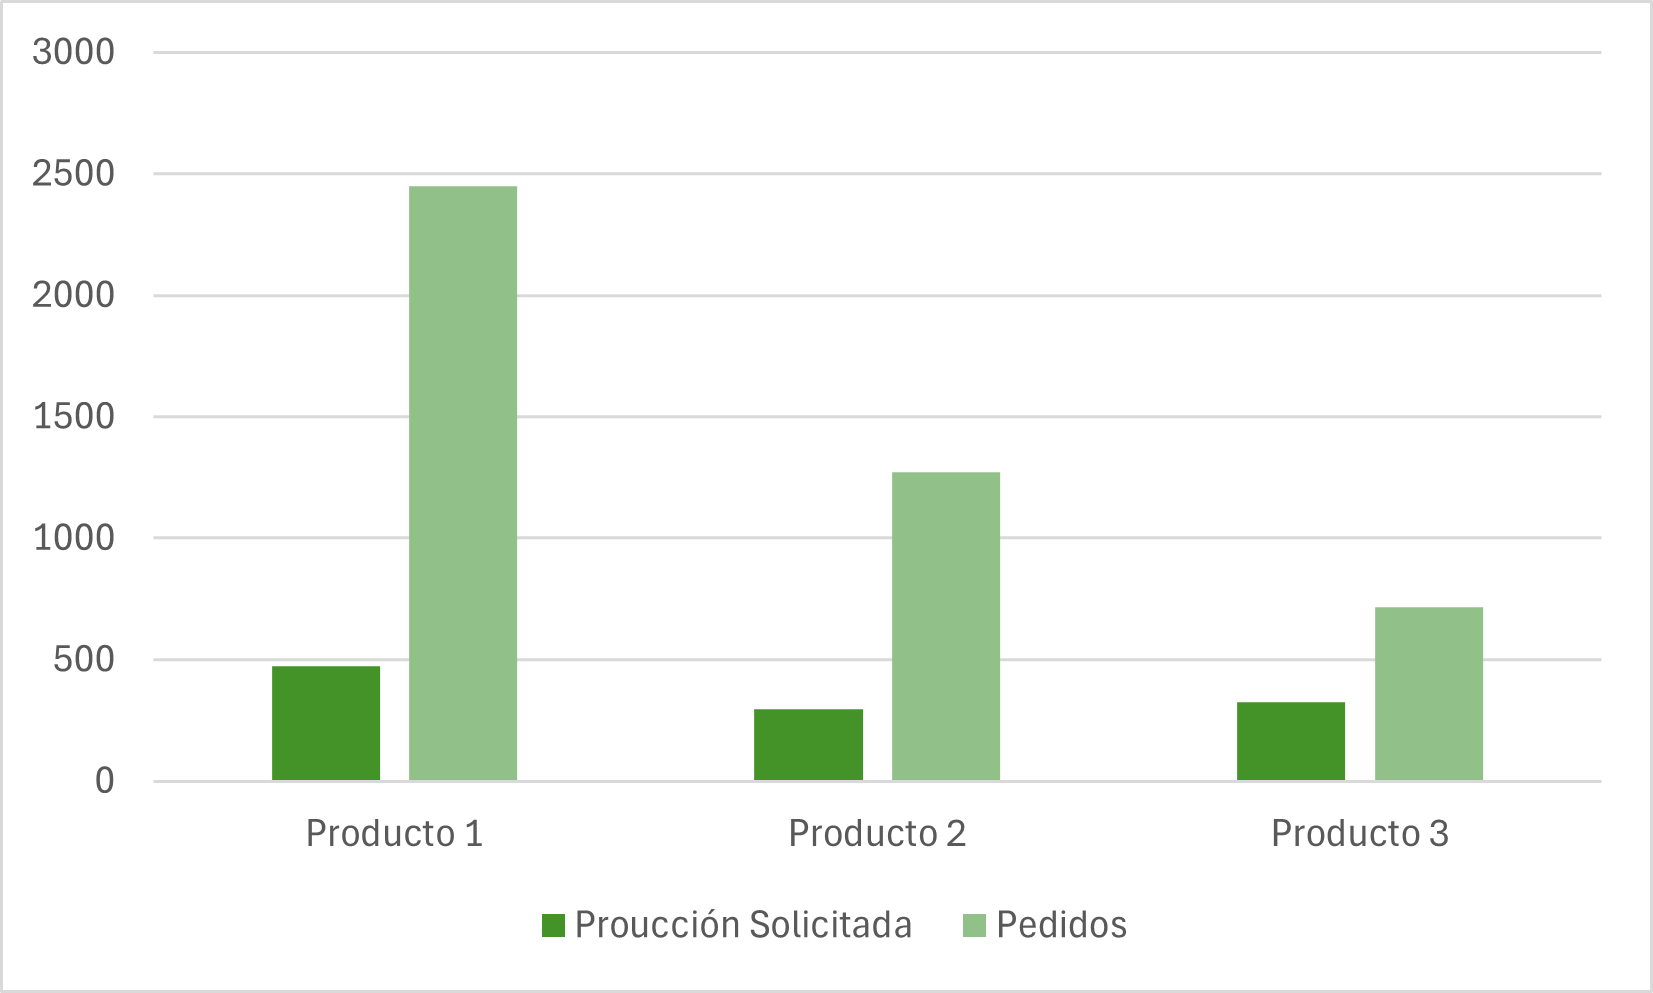
\includegraphics[width= \columnwidth]{Imagenes/decision2_pedidosventas.png}
\end{figure}

Este error de cálculo provocó una ruptura de stock masiva. El mercado europeo, por ejemplo, demandó 1.164 unidades del Producto 1, pero IndusMoney solo pudo entregar 266 unidades. En términos de oportunidad, la empresa dejó de ingresar cientos de miles de euros por pedidos no servidos. Esta infrautilización de la maquinaria y de la mano de obra disponible (que seguía cobrando sus salarios de mecanizado y montaje por valor de 184.311€) disparó el coste unitario de los pocos productos fabricados, destruyendo la rentabilidad operativa. 

En conclusión, se generó una situación de marketing ciego: se invirtió masivamente para atraer clientes a las tiendas (físicas e internet) cuando las estanterías estaban vacías. El resultado es doblemente negativo: 

Por un lado, un dinero que debería haberse destinado a la compra de componentes o mejora de procesos se ha ``quemado´´ en publicidad sin retorno (coste de oportunidad). 

Por otro, el alto nivel de visitas fallidas en la web indica que la demanda frustrada es enorme, lo que supone un daño para la reputación. 

\section*{El Error de Planificación: Infraproducción Crítica}
La raíz del colapso financiero de este trimestre no reside en la falta de clientes, sino en un error de cálculo drástico en la programación de la producción. Mientras que en el trimestre anterior se programó la producción de 1.350 unidades del Producto 1, en esta decisión la cifra se redujo inexplicablemente a 471 unidades. 

Esta decisión de recortar la producción a menos de la mitad, justo cuando se pretendía expandir la marca, dejó a los agentes comerciales con las manos vacías. Por ejemplo, en el mercado europeo para el Producto 1, se recibieron 1.164 pedidos, pero la empresa solo pudo entregar 266 unidades, dejando un enorme volumen de ventas potenciales sin atender y clientes insatisfechos.

\section*{Gasto en Publicidad, pero Nada que Vender}
En un intento por consolidar la marca, el departamento de marketing duplicó la inversión en publicidad, pasando de 101.000€ a 199.000€.  

Esta inversión cumplió su objetivo de atraer clientes, pero al no haber producto disponible, el gasto se transformó en una pérdida neta directa. 

La empresa ha incurrido en una ineficiencia masiva, en la que los costes fijos de mantenimiento, salarios de operarios y la elevada factura publicitaria han devorado el exiguo margen bruto de apenas 58.618€, resultando en unas pérdidas netas de 547.006€. 

\begin{figure}[h]
  \centering
  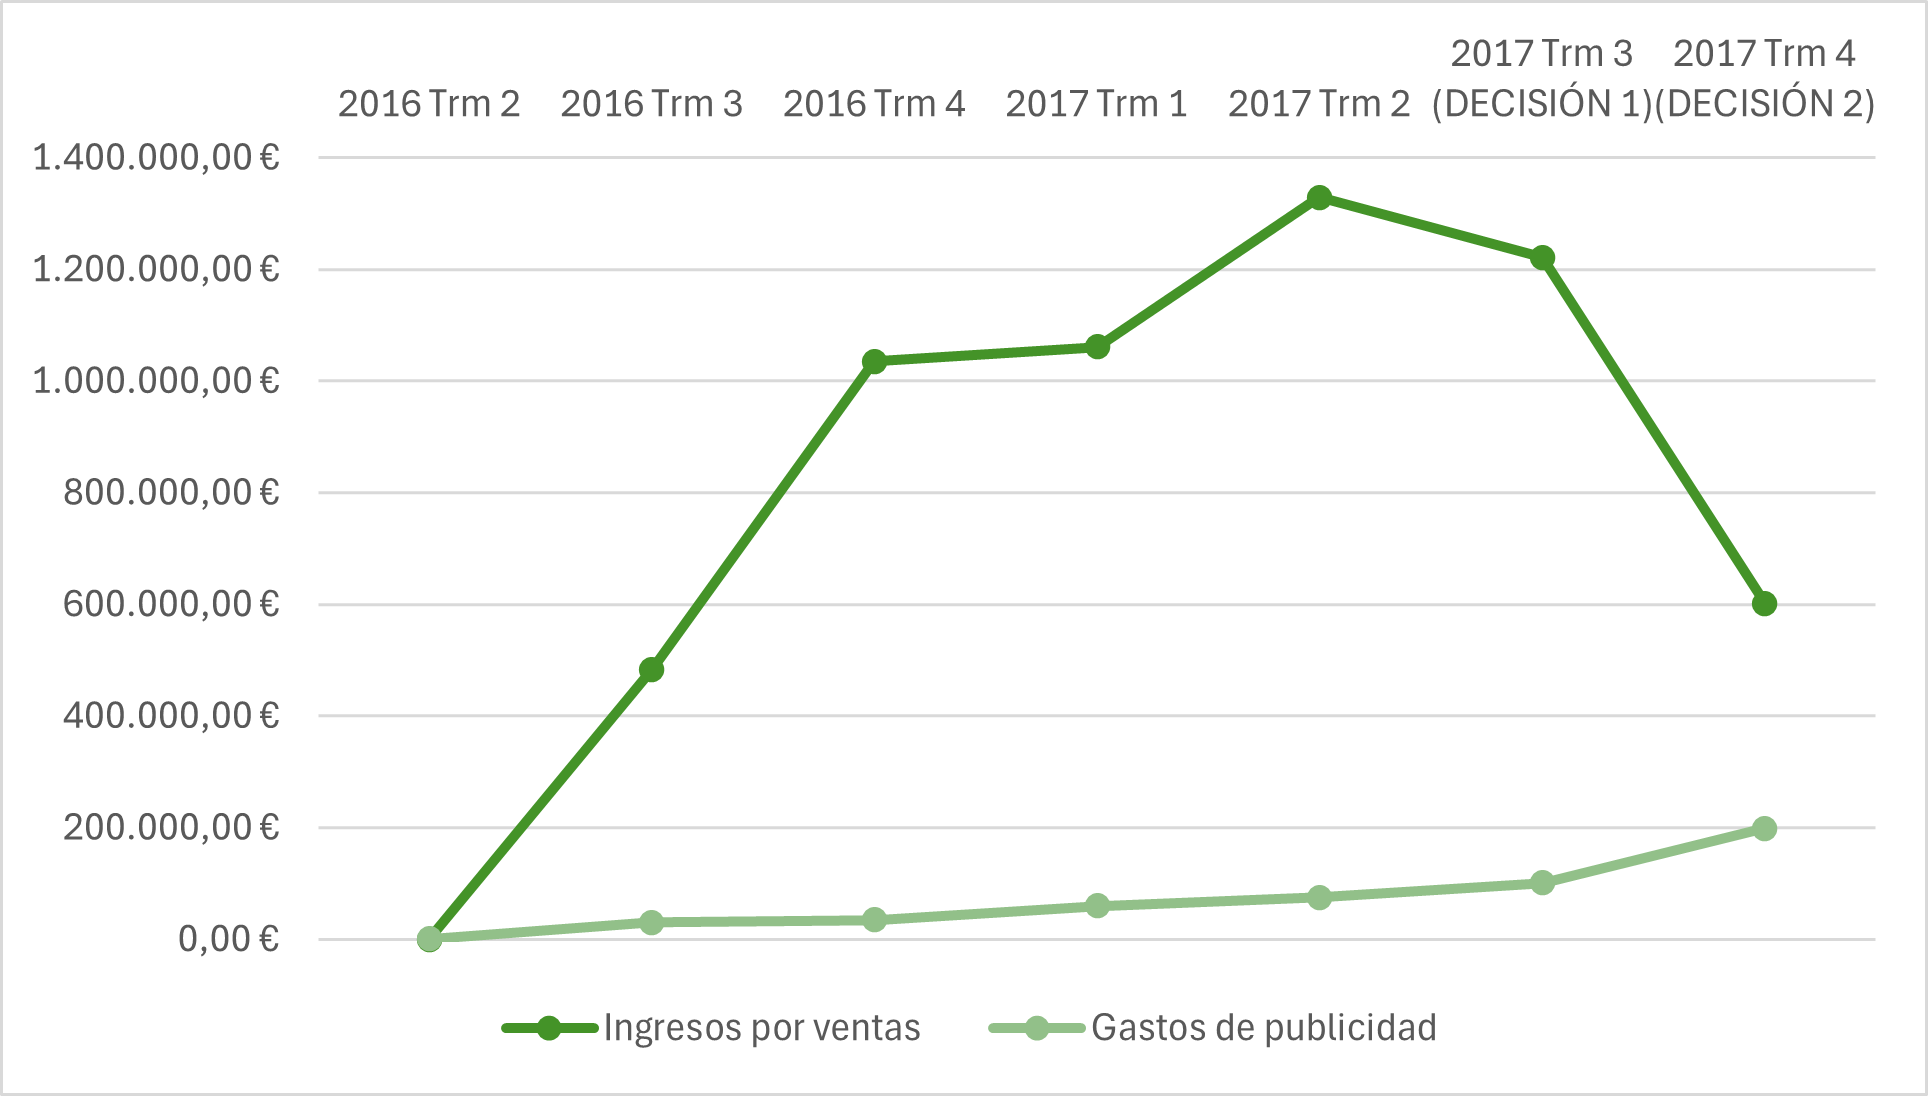
\includegraphics[width= \columnwidth]{Imagenes/decision2_publicidadventas.png}
\end{figure}

\section*{Impacto en el Patrimonio y Solvencia}
La severidad de las pérdidas de este trimestre ha impactado directamente en la solidez del balance. El ROE  se ha hundido hasta el -16,97\%, lo que indica una destrucción acelerada del valor para el accionista. Las reservas acumuladas han pasado a terreno negativo (-776.660€), obligando a la empresa a depender de su capital social para mantenerse a flote. 

La solvencia a corto plazo también se ha visto afectada. Aunque la caja aún mantiene un saldo de 1,5 millones de euros, gran parte de la liquidez está atrapada en un stock de materias primas de 666.702€ que no se está moviendo.  

La rotación de activos (0,13) es la más baja de la historia de la compañía, reflejando que IndusMoney se ha convertido en una estructura pesada e ineficiente que requiere una reestructuración inmediata de sus planes de producción para evitar la insolvencia técnica en los próximos trimestres. 

\section*{El Estrangulamiento Operativo y la Producción}
Como analizamos en la rotación, tener máquinas por valor de más de 1 millón de euros y una plantilla de 45 operarios disponibles para producir apenas 1.100 unidades totales es una ineficiencia masiva. Los salarios de mecanizado y montaje se convierten en un gasto hundido que no genera producto vendible. 

Se reportaron unidades perdidas o destruidas (59 en el P1) debido a la mejora mayor que se implementó en la decisión previa. Esto supuso grandes pérdidas que no fueron compensados por la mejora del producto. 

La baja moral o la falta de incentivos ha provocado que 10 operarios abandonaran la empresa (5 de montaje y 5 de mecanizado). La pérdida de personal cualificado en plena crisis dificulta cualquier intento de reactivación rápida para el T8. 

\section*{La Danza entre la Deuda y el Resguardo del Capital}
La estabilidad de IndusMoney ha pasado de la plenitud a una tensión operativa latente marcada por el retroceso de su liquidez. El Fondo de Maniobra, que alcanzó un máximo de 2.443.045 € en el quinto trimestre, se ha reducido hasta los 1.905.342 € al cierre del séptimo, lo que supone una caída del 20\% en el oxígeno financiero necesario para operar sin comprometer los activos fijos de la compañía.

\begin{figure}[h]
  \centering
  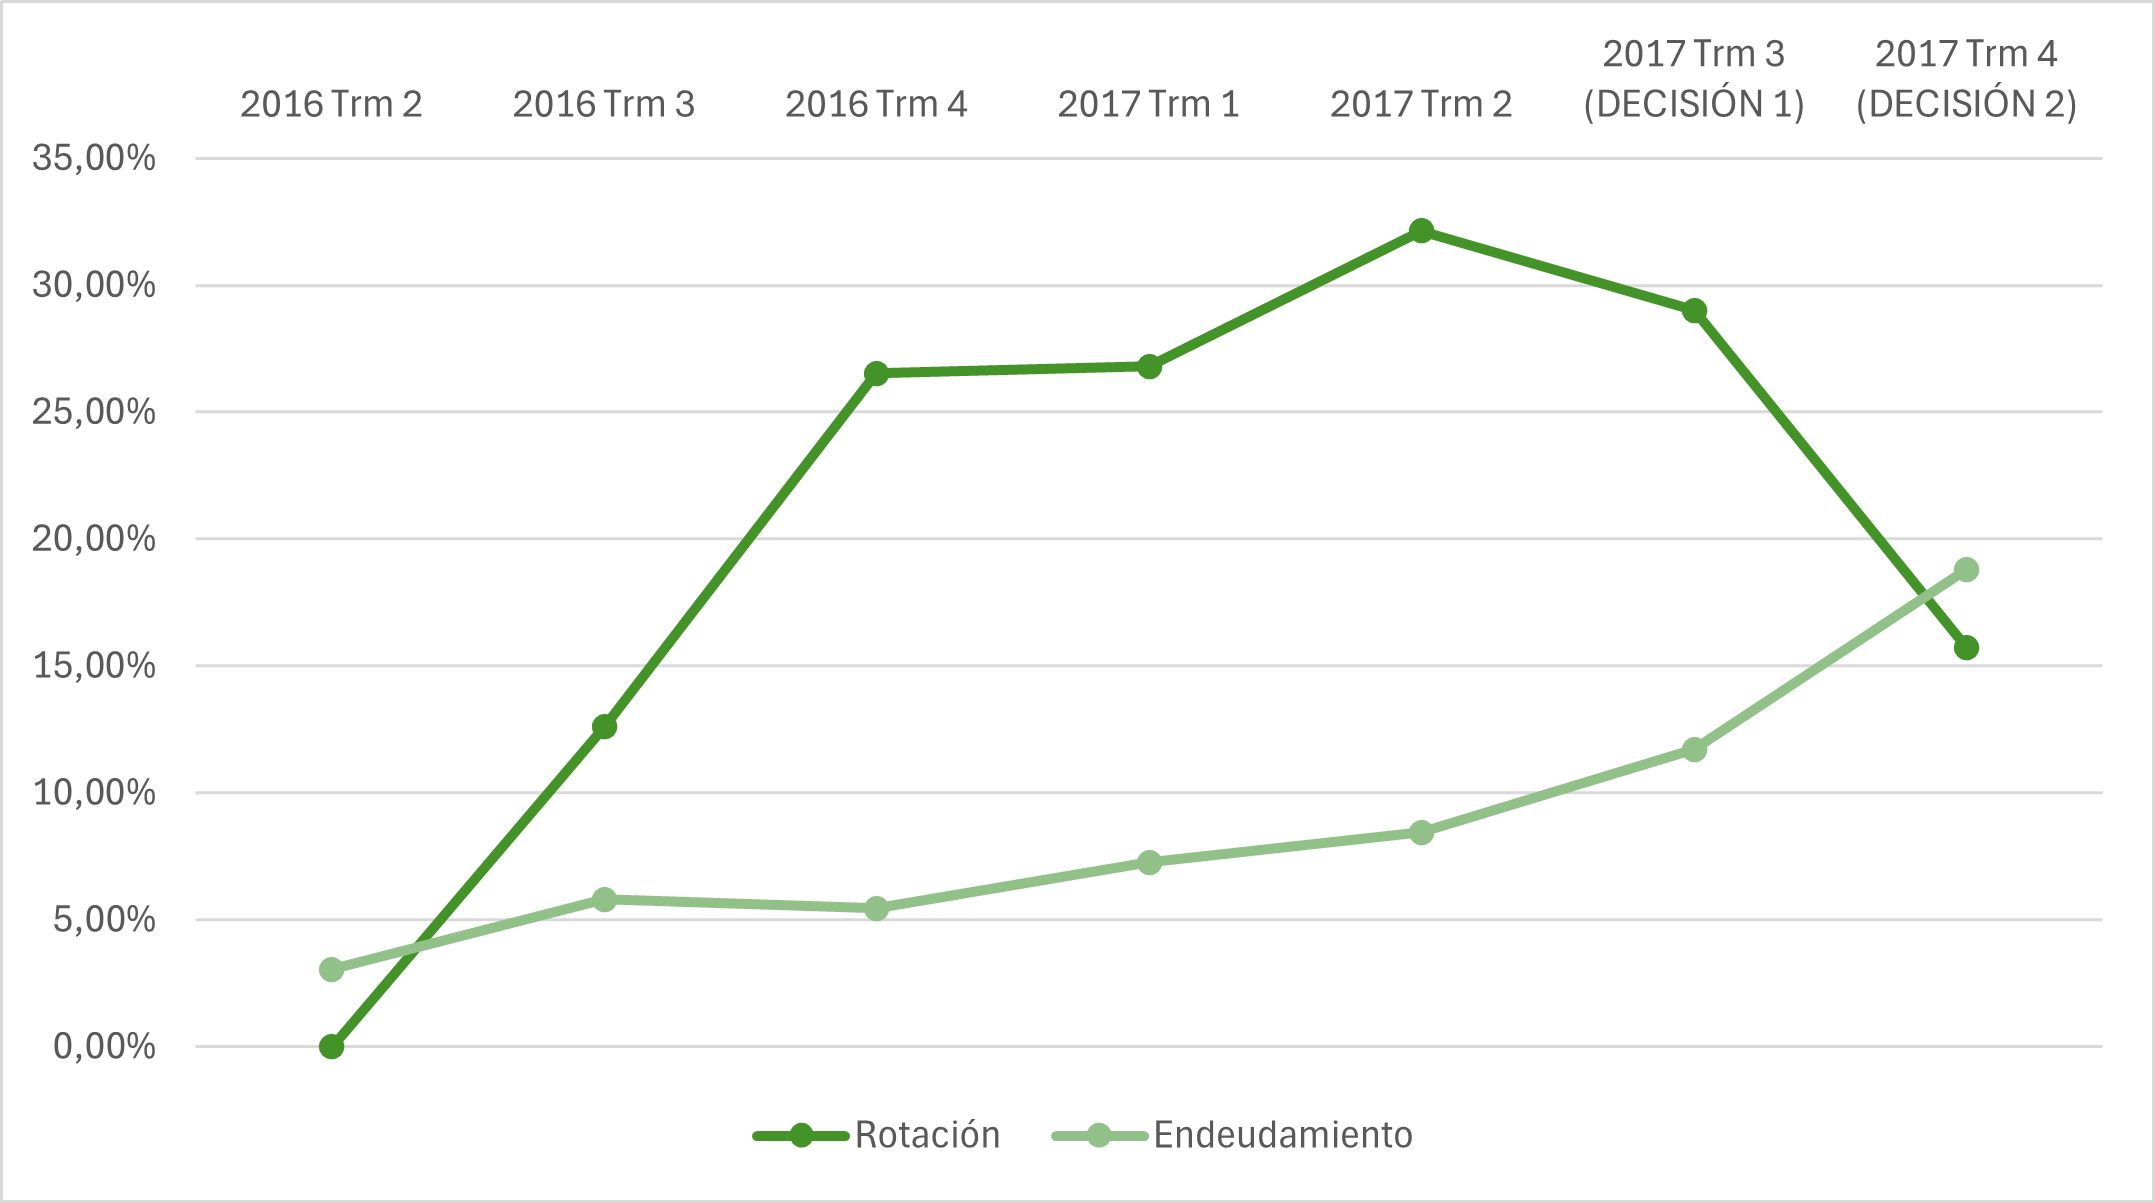
\includegraphics[width= \columnwidth]{Imagenes/decision2_endeudamiento.png}
\end{figure}

Esta erosión nace de un capital cautivo en materias primas por 666.702 € y un pasivo corriente que ha escalado hasta los 606.061 €. Como resultado, la ratio de endeudamiento ha saltado del 7,7\% al 15,8\%, reflejando una dependencia creciente de la financiación ajena para sostener una estructura productiva que, en el último periodo, no ha generado el flujo de caja suficiente para sanear sus deudas comerciales.

\section*{El Latido Herido del Rendimiento del Accionista}
La rentabilidad sobre los fondos propios o ROE ha sufrido un impacto devastador como reflejo directo de la ineficiencia operativa del séptimo trimestre. Ha pasado de un terreno positivo a una destrucción de valor para el accionista sin precedentes en la serie histórica. 

Mientras que en el quinto trimestre la compañía lograba una rentabilidad del 3,18\%, el cierre del séptimo trimestre arroja una cifra alarmante del 16,97\% negativo, lo que indica que por cada euro de capital invertido la empresa está perdiendo casi 17 céntimos debido a la magnitud de las pérdidas netas de 547.006 €.

\begin{figure}[h]
  \centering
  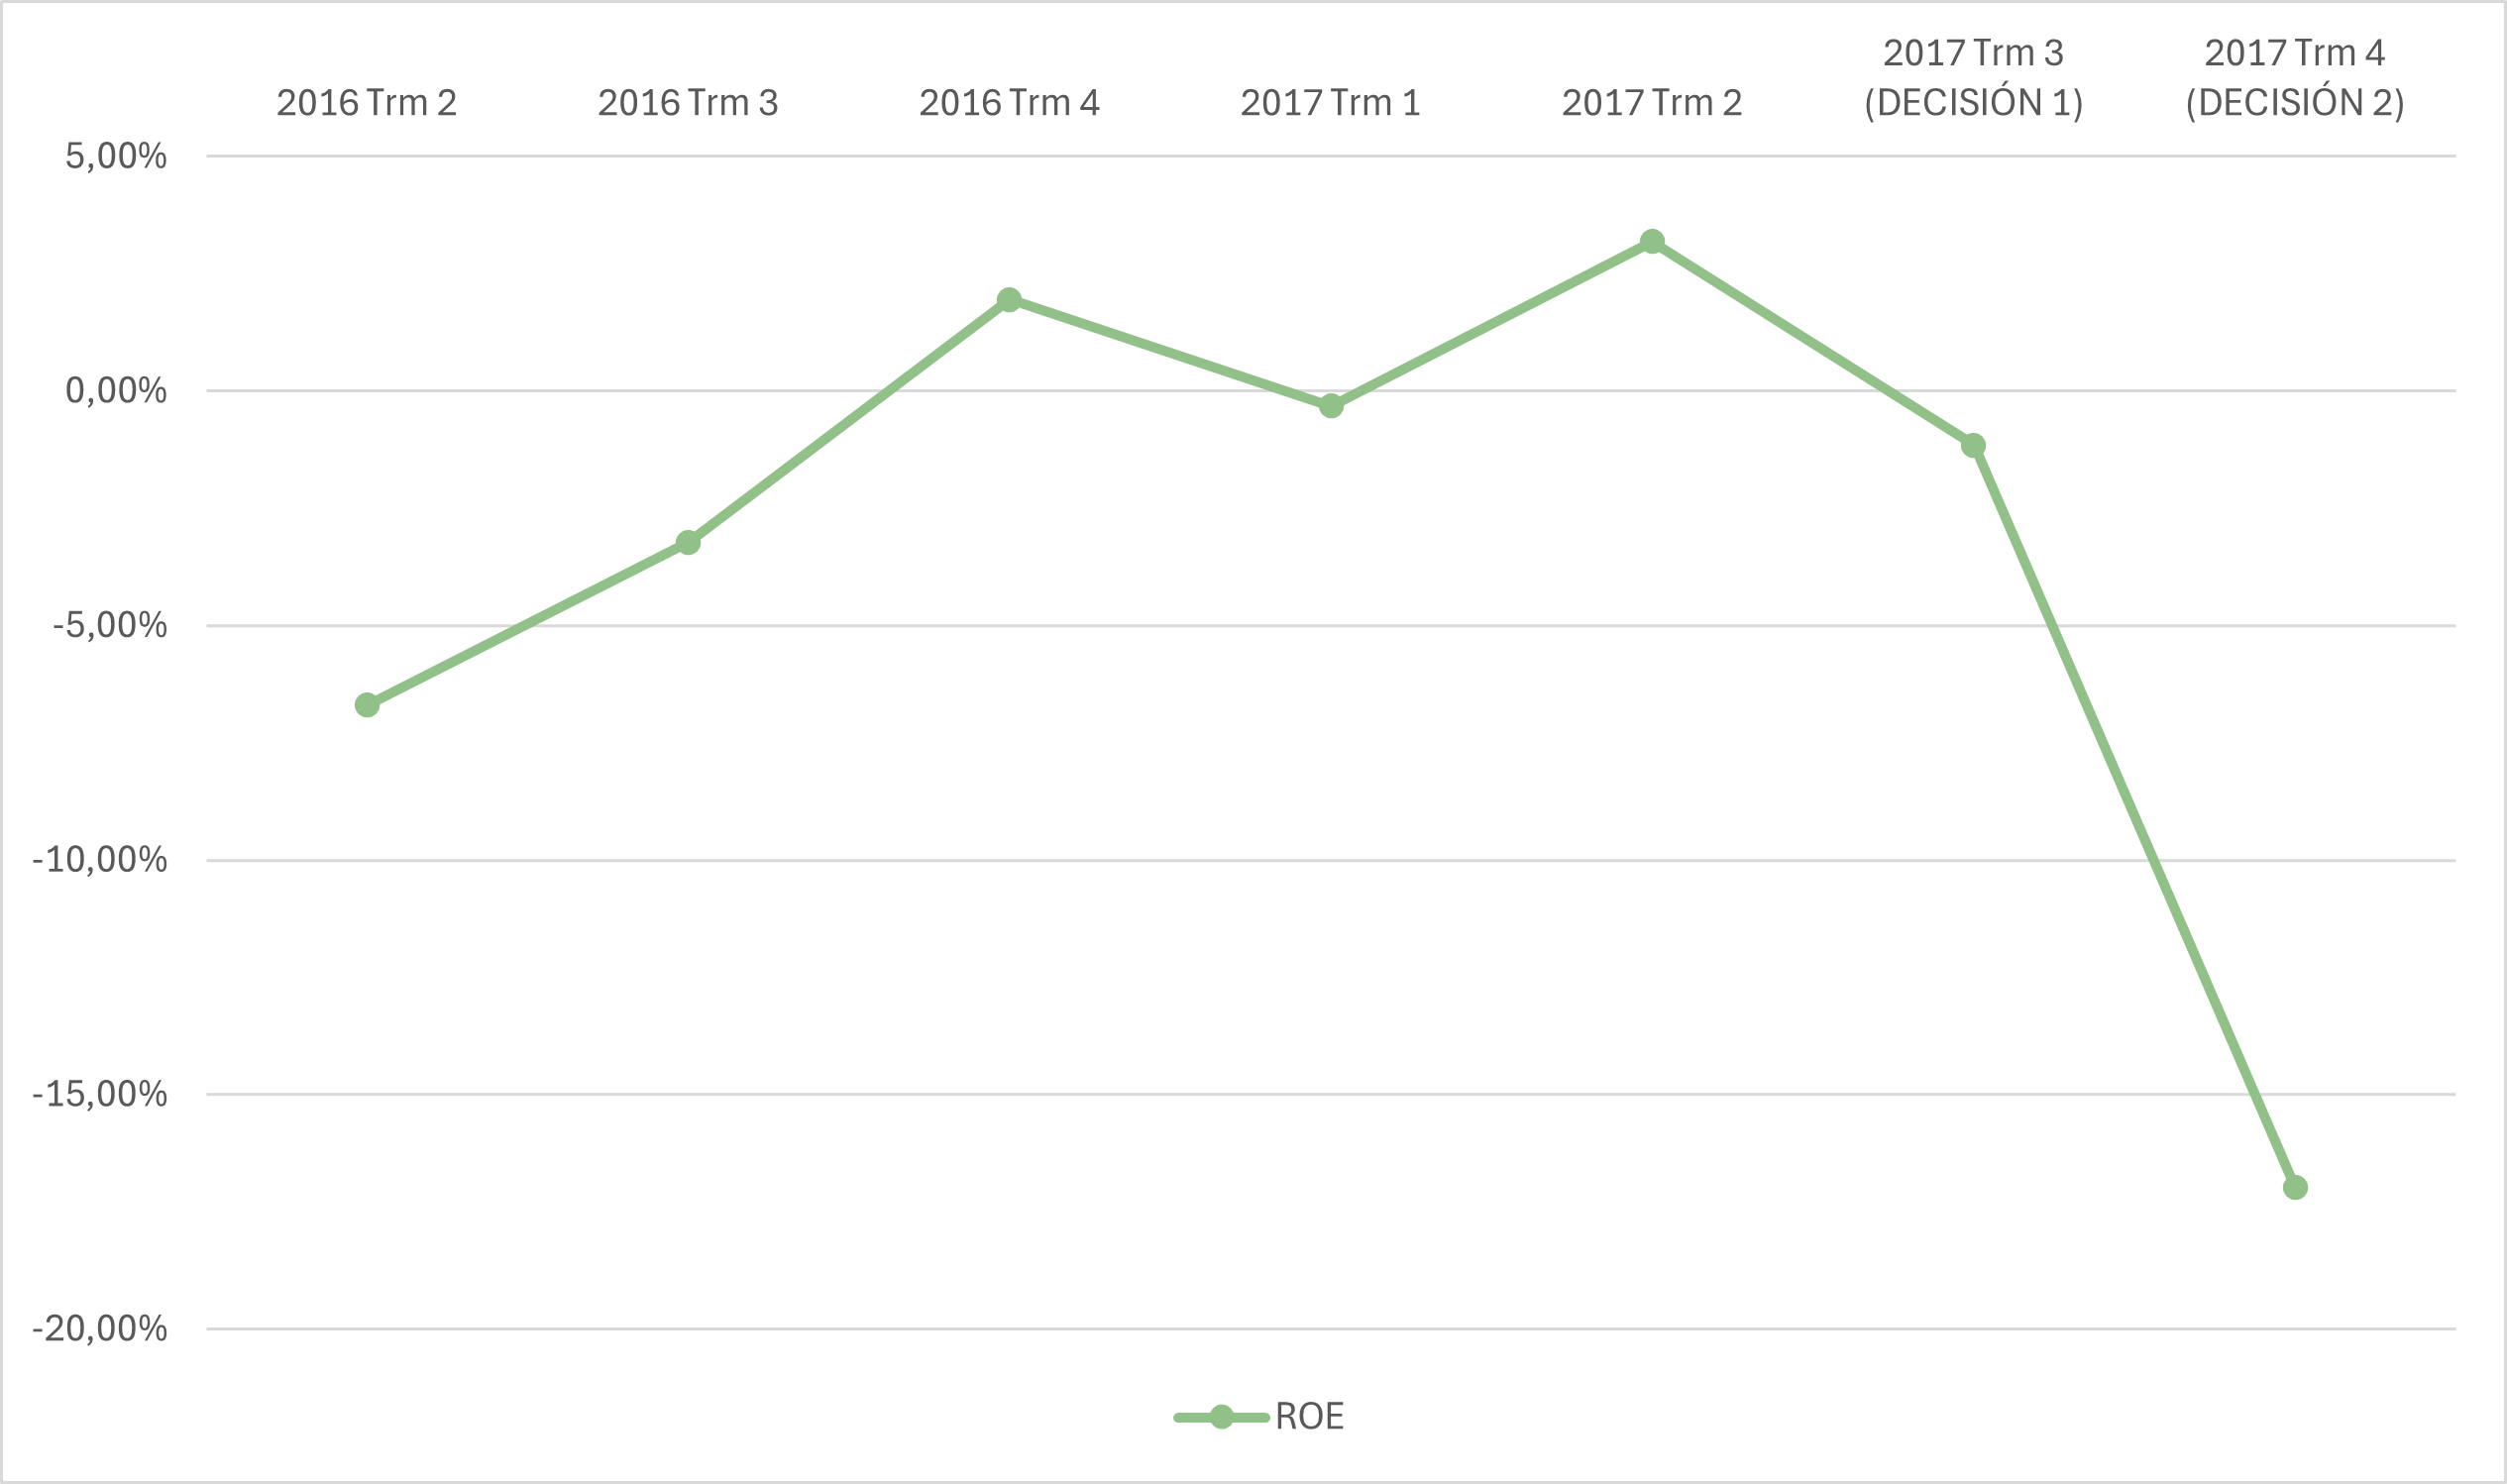
\includegraphics[width= \columnwidth]{Imagenes/decision2_ROE.png}
\end{figure}

Recuperar un ROE positivo en el octavo trimestre dependerá exclusivamente de la capacidad de la dirección para reactivar la producción masiva, ya que cualquier incremento adicional en el endeudamiento para cubrir pérdidas solo serviría para apalancar negativamente a la empresa y comprometer la viabilidad de IndusMoney en la competición.

\section*{Plan de Emergencia}
El Trimestre 7 ha sido un error de descoordinación logística. IndusMoney se comportó como una empresa comercial agresiva teniendo la fábrica de una empresa artesanal. 

Para evitarlo, se la nueva línea de acción fue la siguiente: 
\begin{enumerate}
    \item Se debe programar la máxima capacidad de la fábrica. Es preferible acumular stock que tener a los operarios de brazos cruzados. 
    \item La marca ya tiene inercia. Es necesario bajar el gasto publicitario a niveles de 70k-80k€. 
    \item Es crítico volver a contratar y formar personal inmediatamente para compensar las 10 bajas. 
\end{enumerate}


\begin{table}[h]
    \centering
    \begin{tabular}{lr}
        \textbf{Balance - 2ª Decisión}               & \textbf{€} \\
        \hline
        \textbf{Activo fijo}                & \\
        Terreno                             & 50000 \\
        Bienes inmuebles                    & 250000 \\
        Valor de las máquinas               & 1017998 \\
        \cline{2-2}
        \textbf{Total activo fijo}          & \textbf{1317998} \\
        \textbf{Activo Circulante}          & \\
        Inventario - Productos              & 0 \\
        Inventario - Componentes            & 24570 \\
        Inventario - Materia Prima          & 666702 \\
        Deudores                            & 314042 \\
        Efectivo e Inversores               & 1506089 \\
        \cline{2-2}
        \textbf{Total activo circulante}    & \textbf{2511403} \\
        \cline{2-2}
        \textbf{Activo Total}               & \textbf{3829401} \\
        \textbf{Pasivo:}                    & \\
        Impuestos a pagar                   & 0 \\
        Acreedores                          & 606061 \\
        Línea de crédito / Descubierto      & 0 \\
        \cline{2-2}
        \textbf{Pasivo exigible}            & \textbf{606061} \\
        \textbf{Préstamos}                  & \textbf{0} \\
        \textbf{Activo neto}                & \textbf{3223340} \\
        \textbf{Fondos propios}             & \\
        Capital social                      & 4000000 \\
        Prima de emisión                    & 0 \\
        Reservas                            & -776660 \\
        \cline{2-2}
        \textbf{Patrimonio neto}            & 3223340 
    \end{tabular}
\end{table}

\begin{table}[h]
    \centering
    \begin{tabular}{|c|r|}
        \hline
        NOF & 1.905.342,00 € \\
        FM & -1.317.998,00 € \\
        EC & -3.223.340,00 € \\
        \hline
    \end{tabular}
\end{table}